\begin{figure}[p]
\centering\renewcommand{\figurename}{Supplementary Figure}\renewcommand{\thefigure}{S1}%
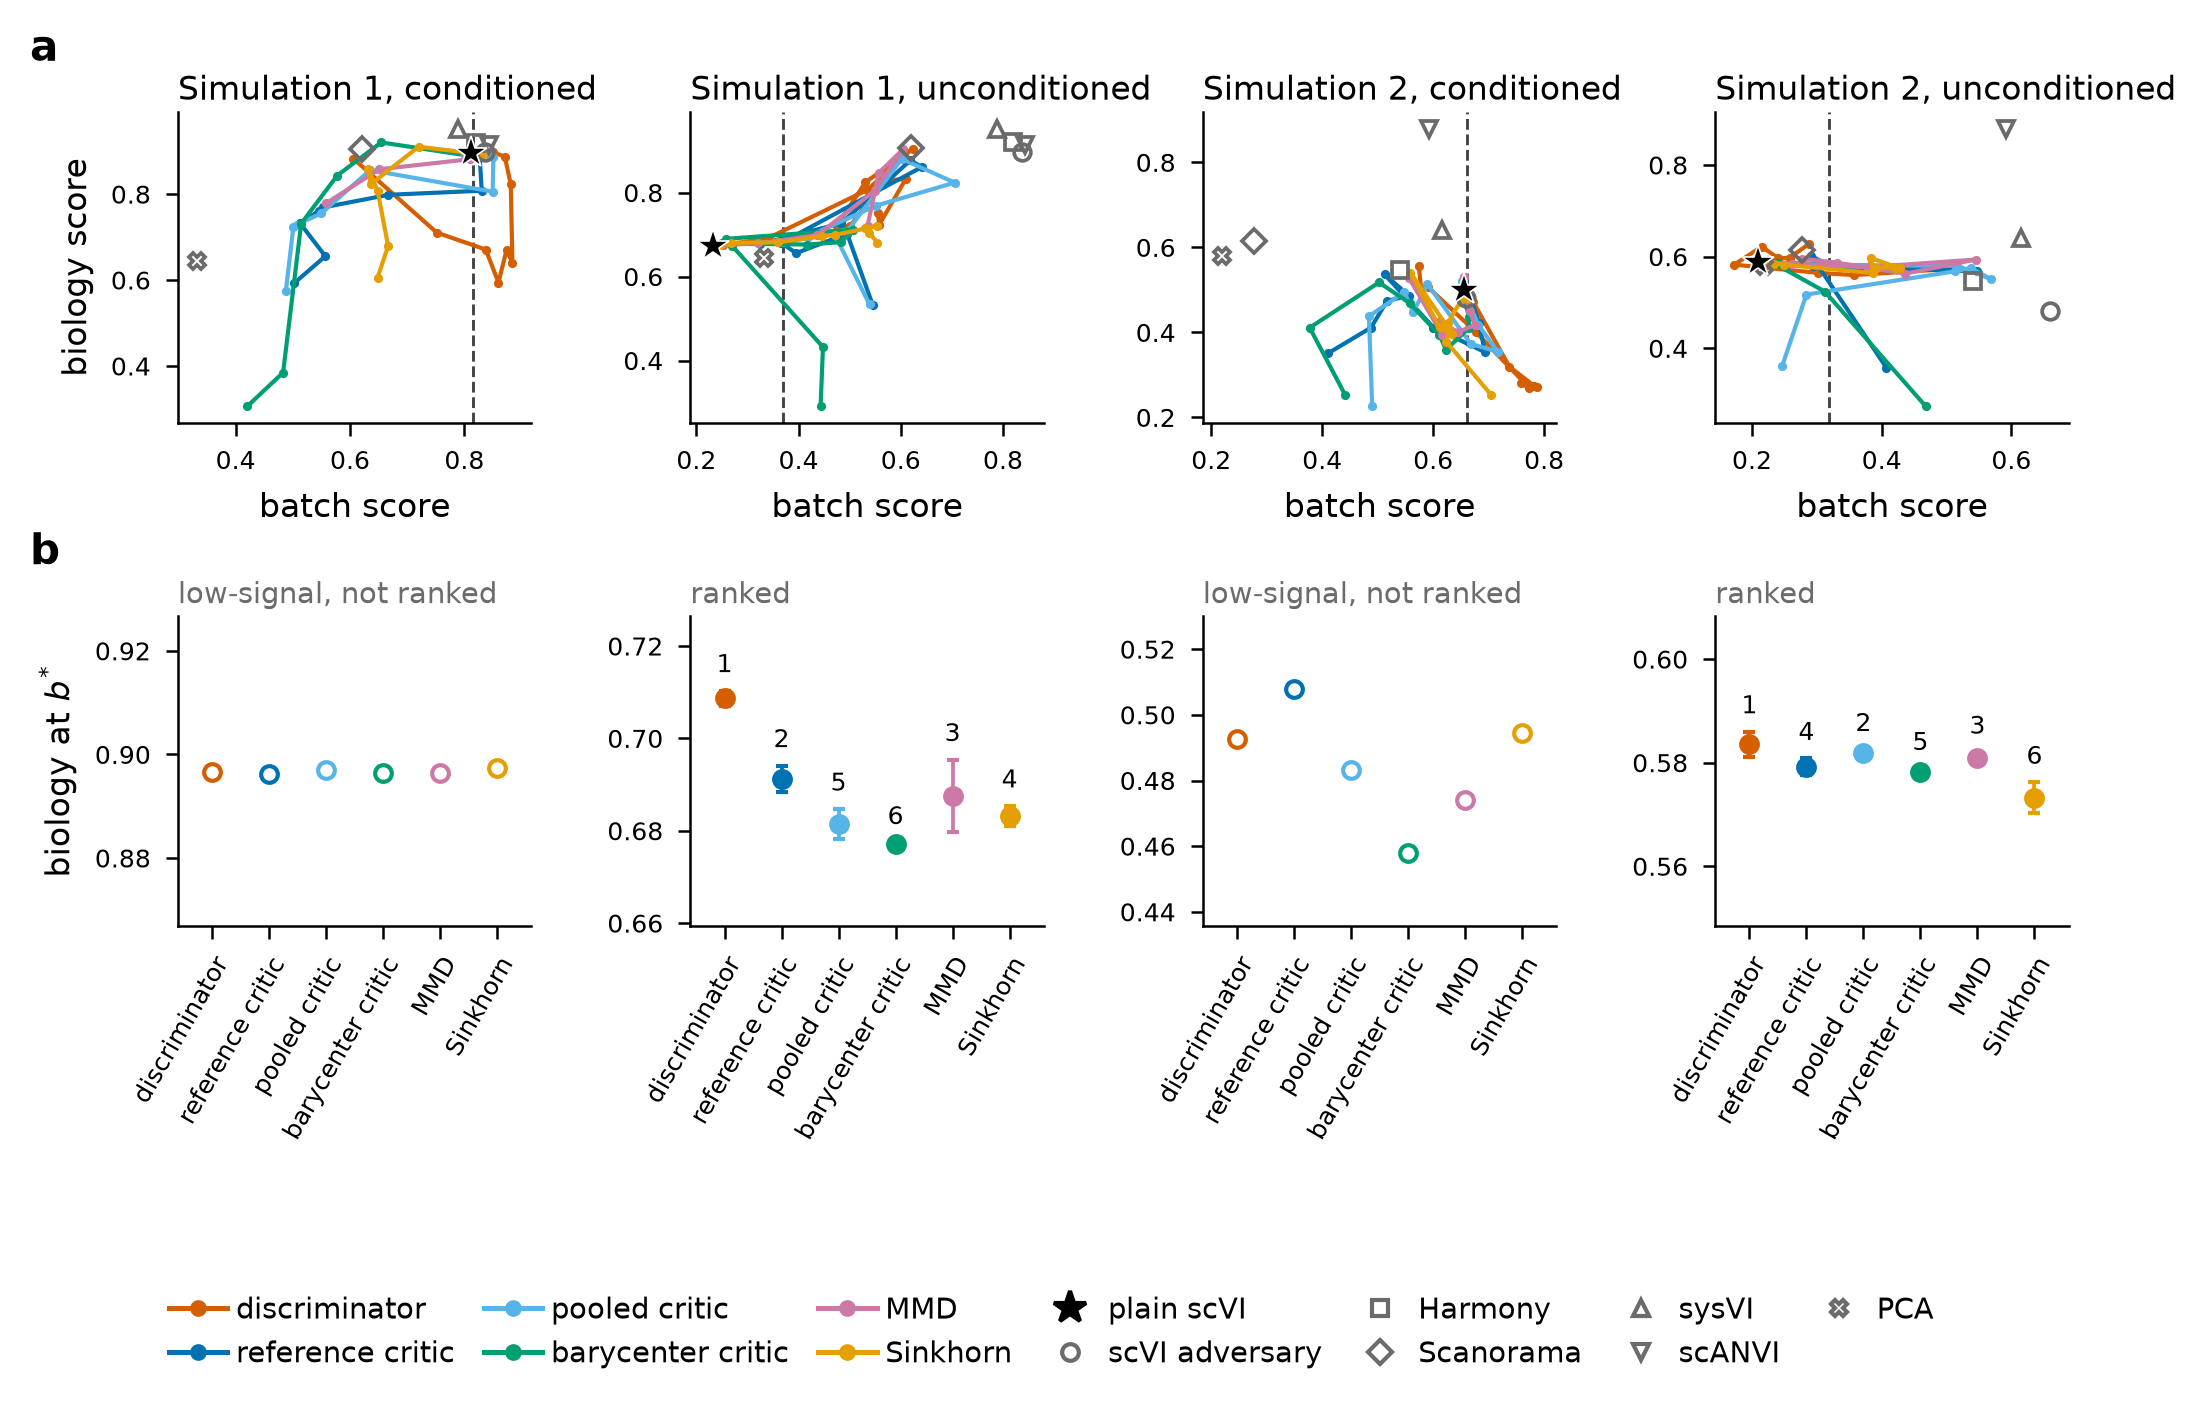
\includegraphics[width=\textwidth]{figures/figS1.png}
\caption{Simulation tasks with both decoders. \textbf{(a)} Seed-mean batch and biology scores across strengths, with plain scVI as a star, $b^*$ dashed and each standard tool's best selection-score setting in grey. \textbf{(b)} Biology at $b^*$ with leave-one-seed-out errors and ranks. Open markers identify low-signal batch-conditioned simulations, shown without errors or ranks. Simulations are ranked separately from real tasks (Supplementary Notes 5 and 6).}\label{fig:s1}
\end{figure}

\begin{figure}[p]
\centering\renewcommand{\figurename}{Supplementary Figure}\renewcommand{\thefigure}{S2}%
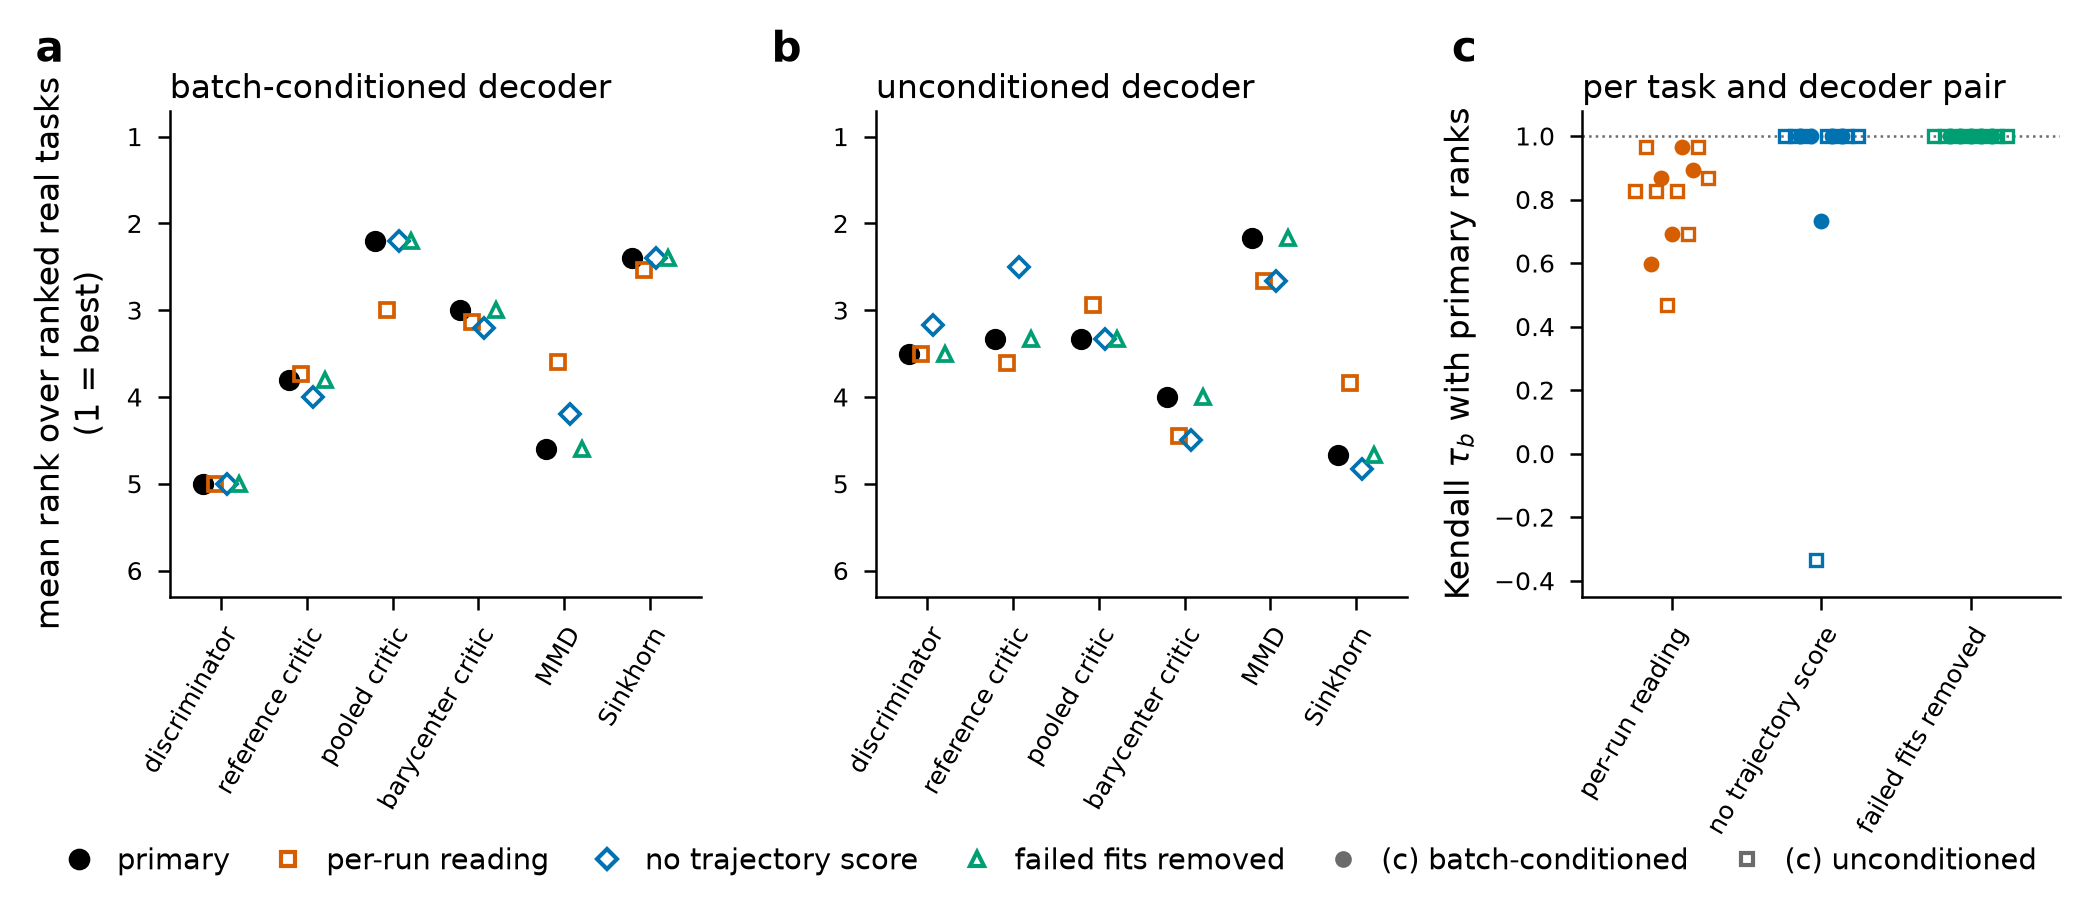
\includegraphics[width=\textwidth]{figures/figS2.png}
\caption{Sensitivity of rankings to per-seed readings, omission of trajectory conservation and removal of strengths containing failed fits. The last reproduces primary ranks because no fit failed. \textbf{(a, b)} Mean ranks across ranked real tasks by decoder. \textbf{(c)} Kendall's $\tau_b$ against primary ranks in each of 13 ranked pairs, including simulations. Points at 1 overlap (Supplementary Note 6).}\label{fig:s2}
\end{figure}

\begin{figure}[p]
\centering\renewcommand{\figurename}{Supplementary Figure}\renewcommand{\thefigure}{S3}%
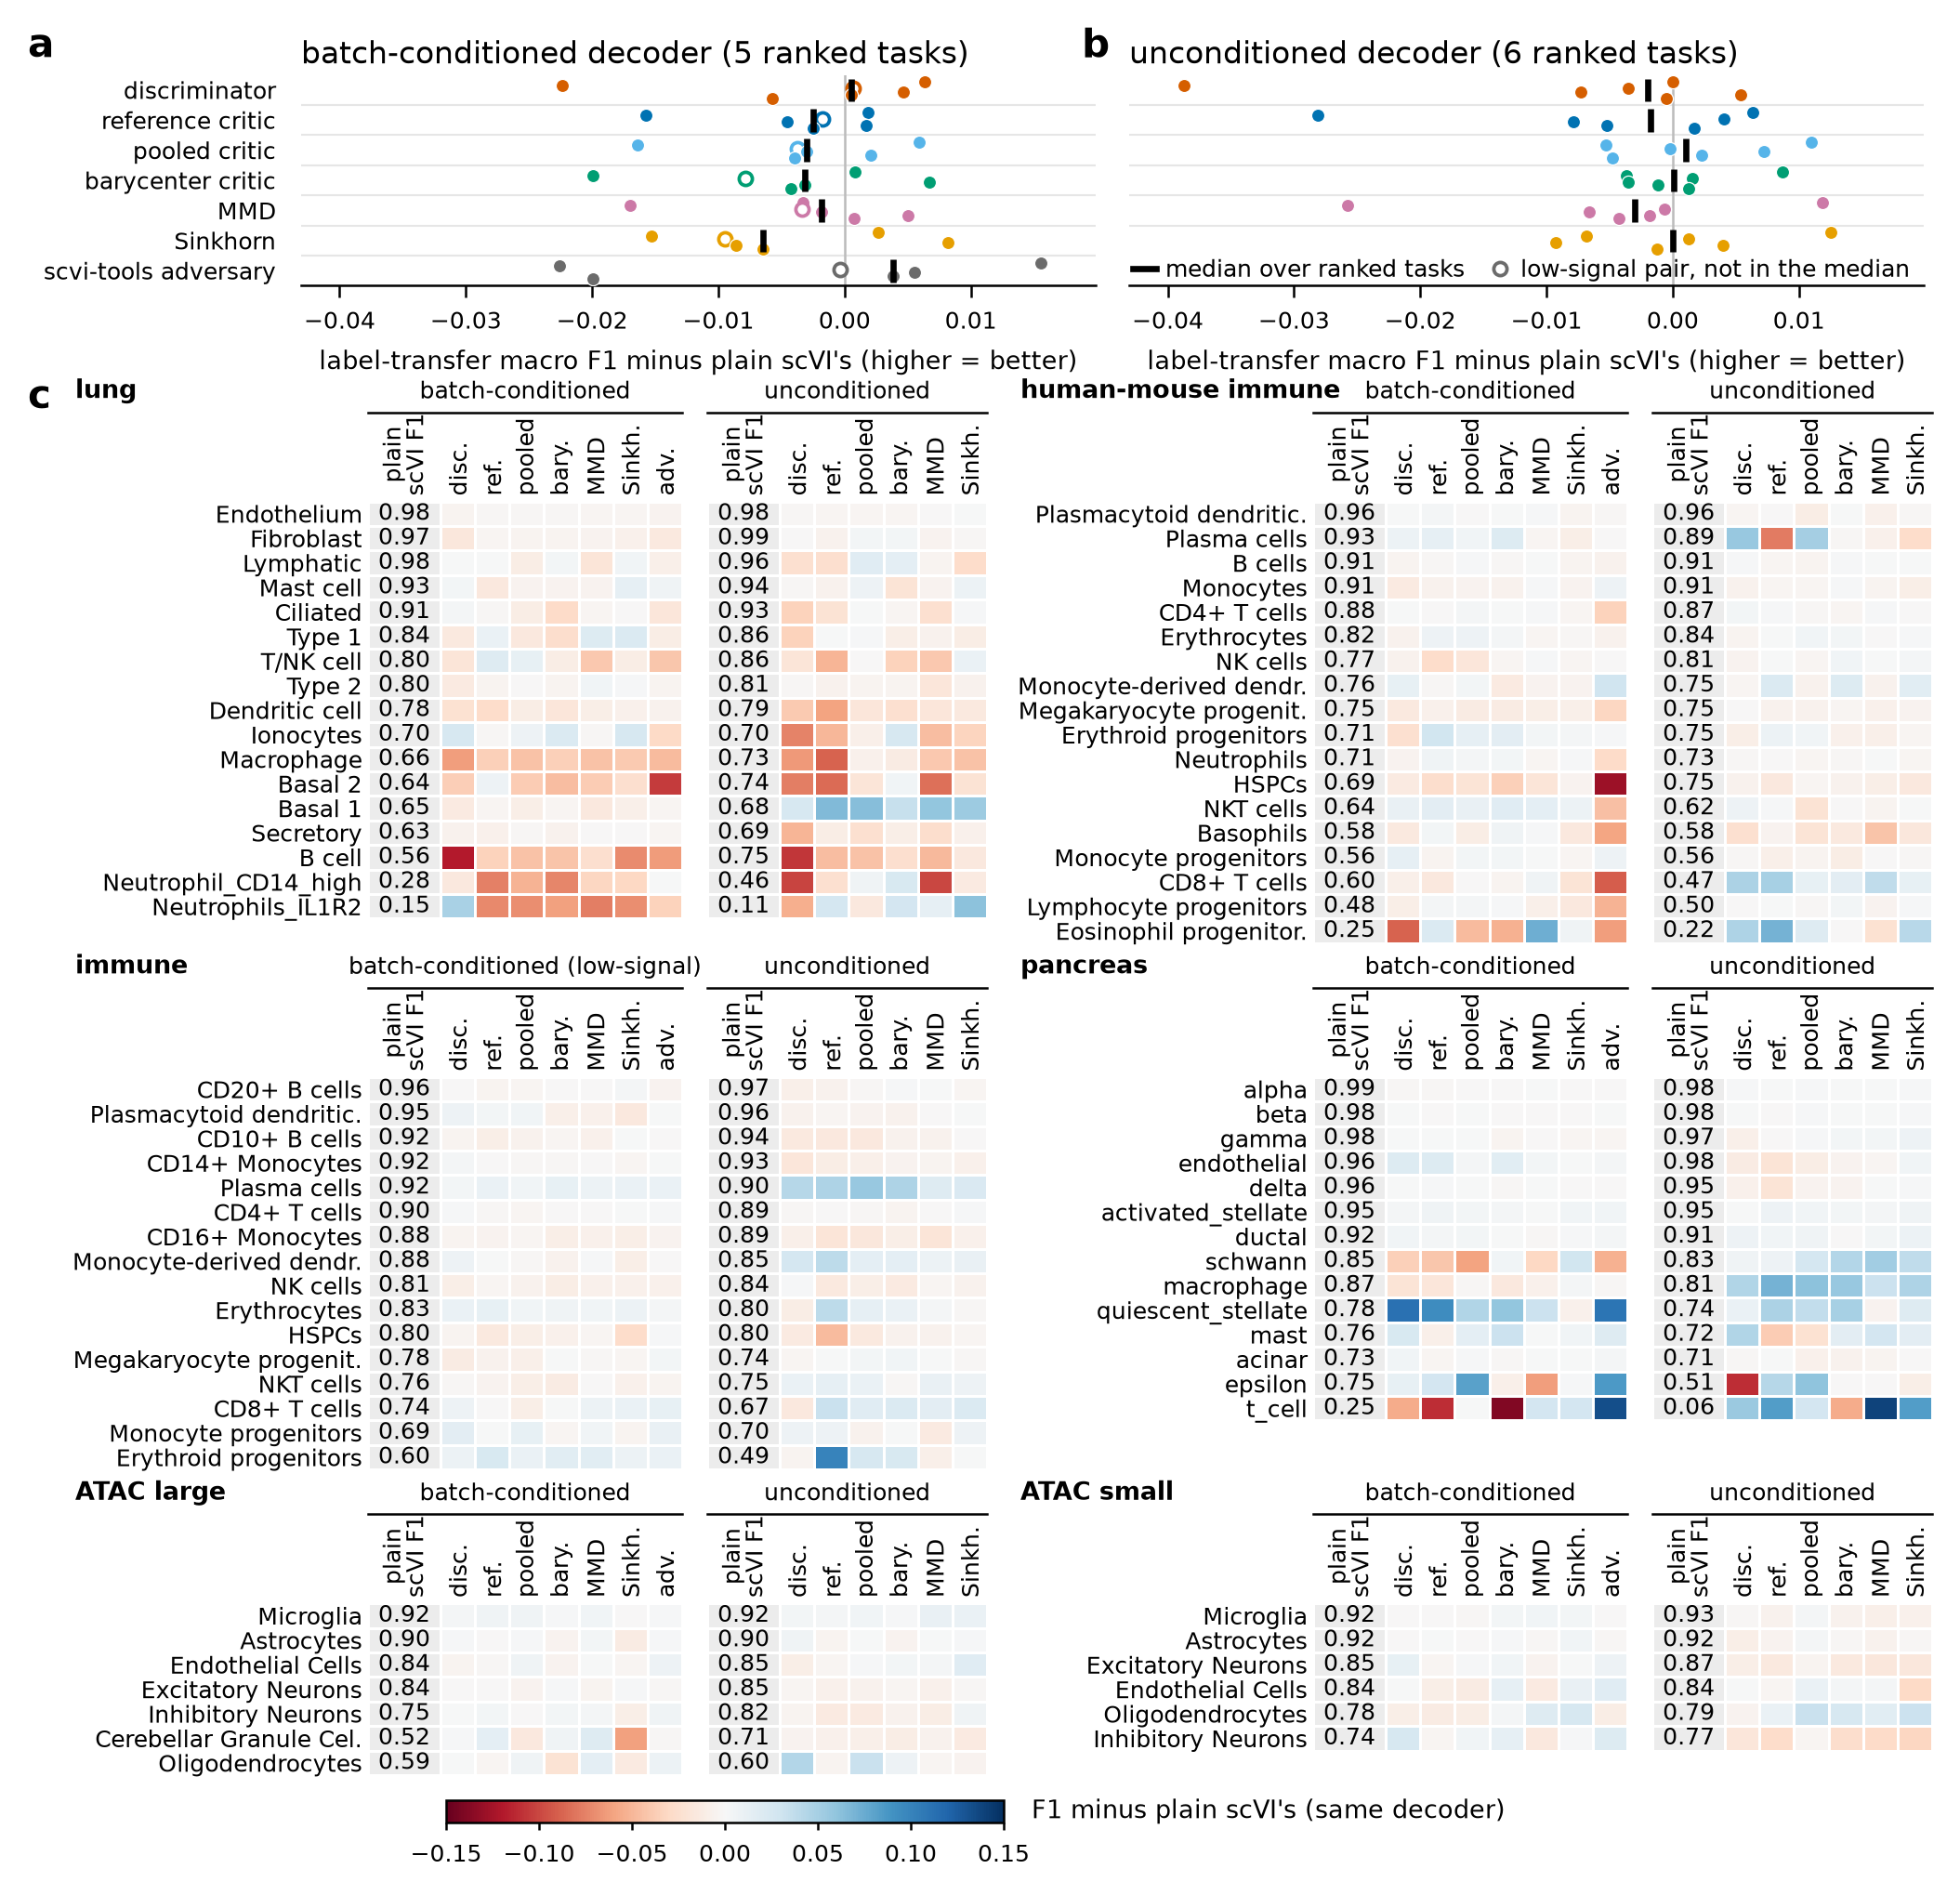
\includegraphics[width=\textwidth,height=0.76\textheight,keepaspectratio]{figures/figS3.png}
\caption{Label transfer at first-crossing strengths on real tasks (Supplementary Note 9). Plain scVI and the scvi-tools adversary are unmatched. \textbf{(a, b)} Macro-F1 differences from same-decoder plain scVI for batch-conditioned and unconditioned models. Dots are tasks; black ticks are ranked-task medians. The open immune dot is low-signal and excluded from its median. \textbf{(c)} Per-type F1 averaged over held-out batches and seeds. Grey shows plain scVI; colours show differences, blue above and red below, limited to $\pm0.15$. Types are ordered by plain-scVI F1. Abbreviations denote discriminator, reference critic, barycenter critic, Sinkhorn divergence and scvi-tools adversary.}\label{fig:s3}
\end{figure}

\begin{figure}[p]
\centering\renewcommand{\figurename}{Supplementary Figure}\renewcommand{\thefigure}{S4a}%
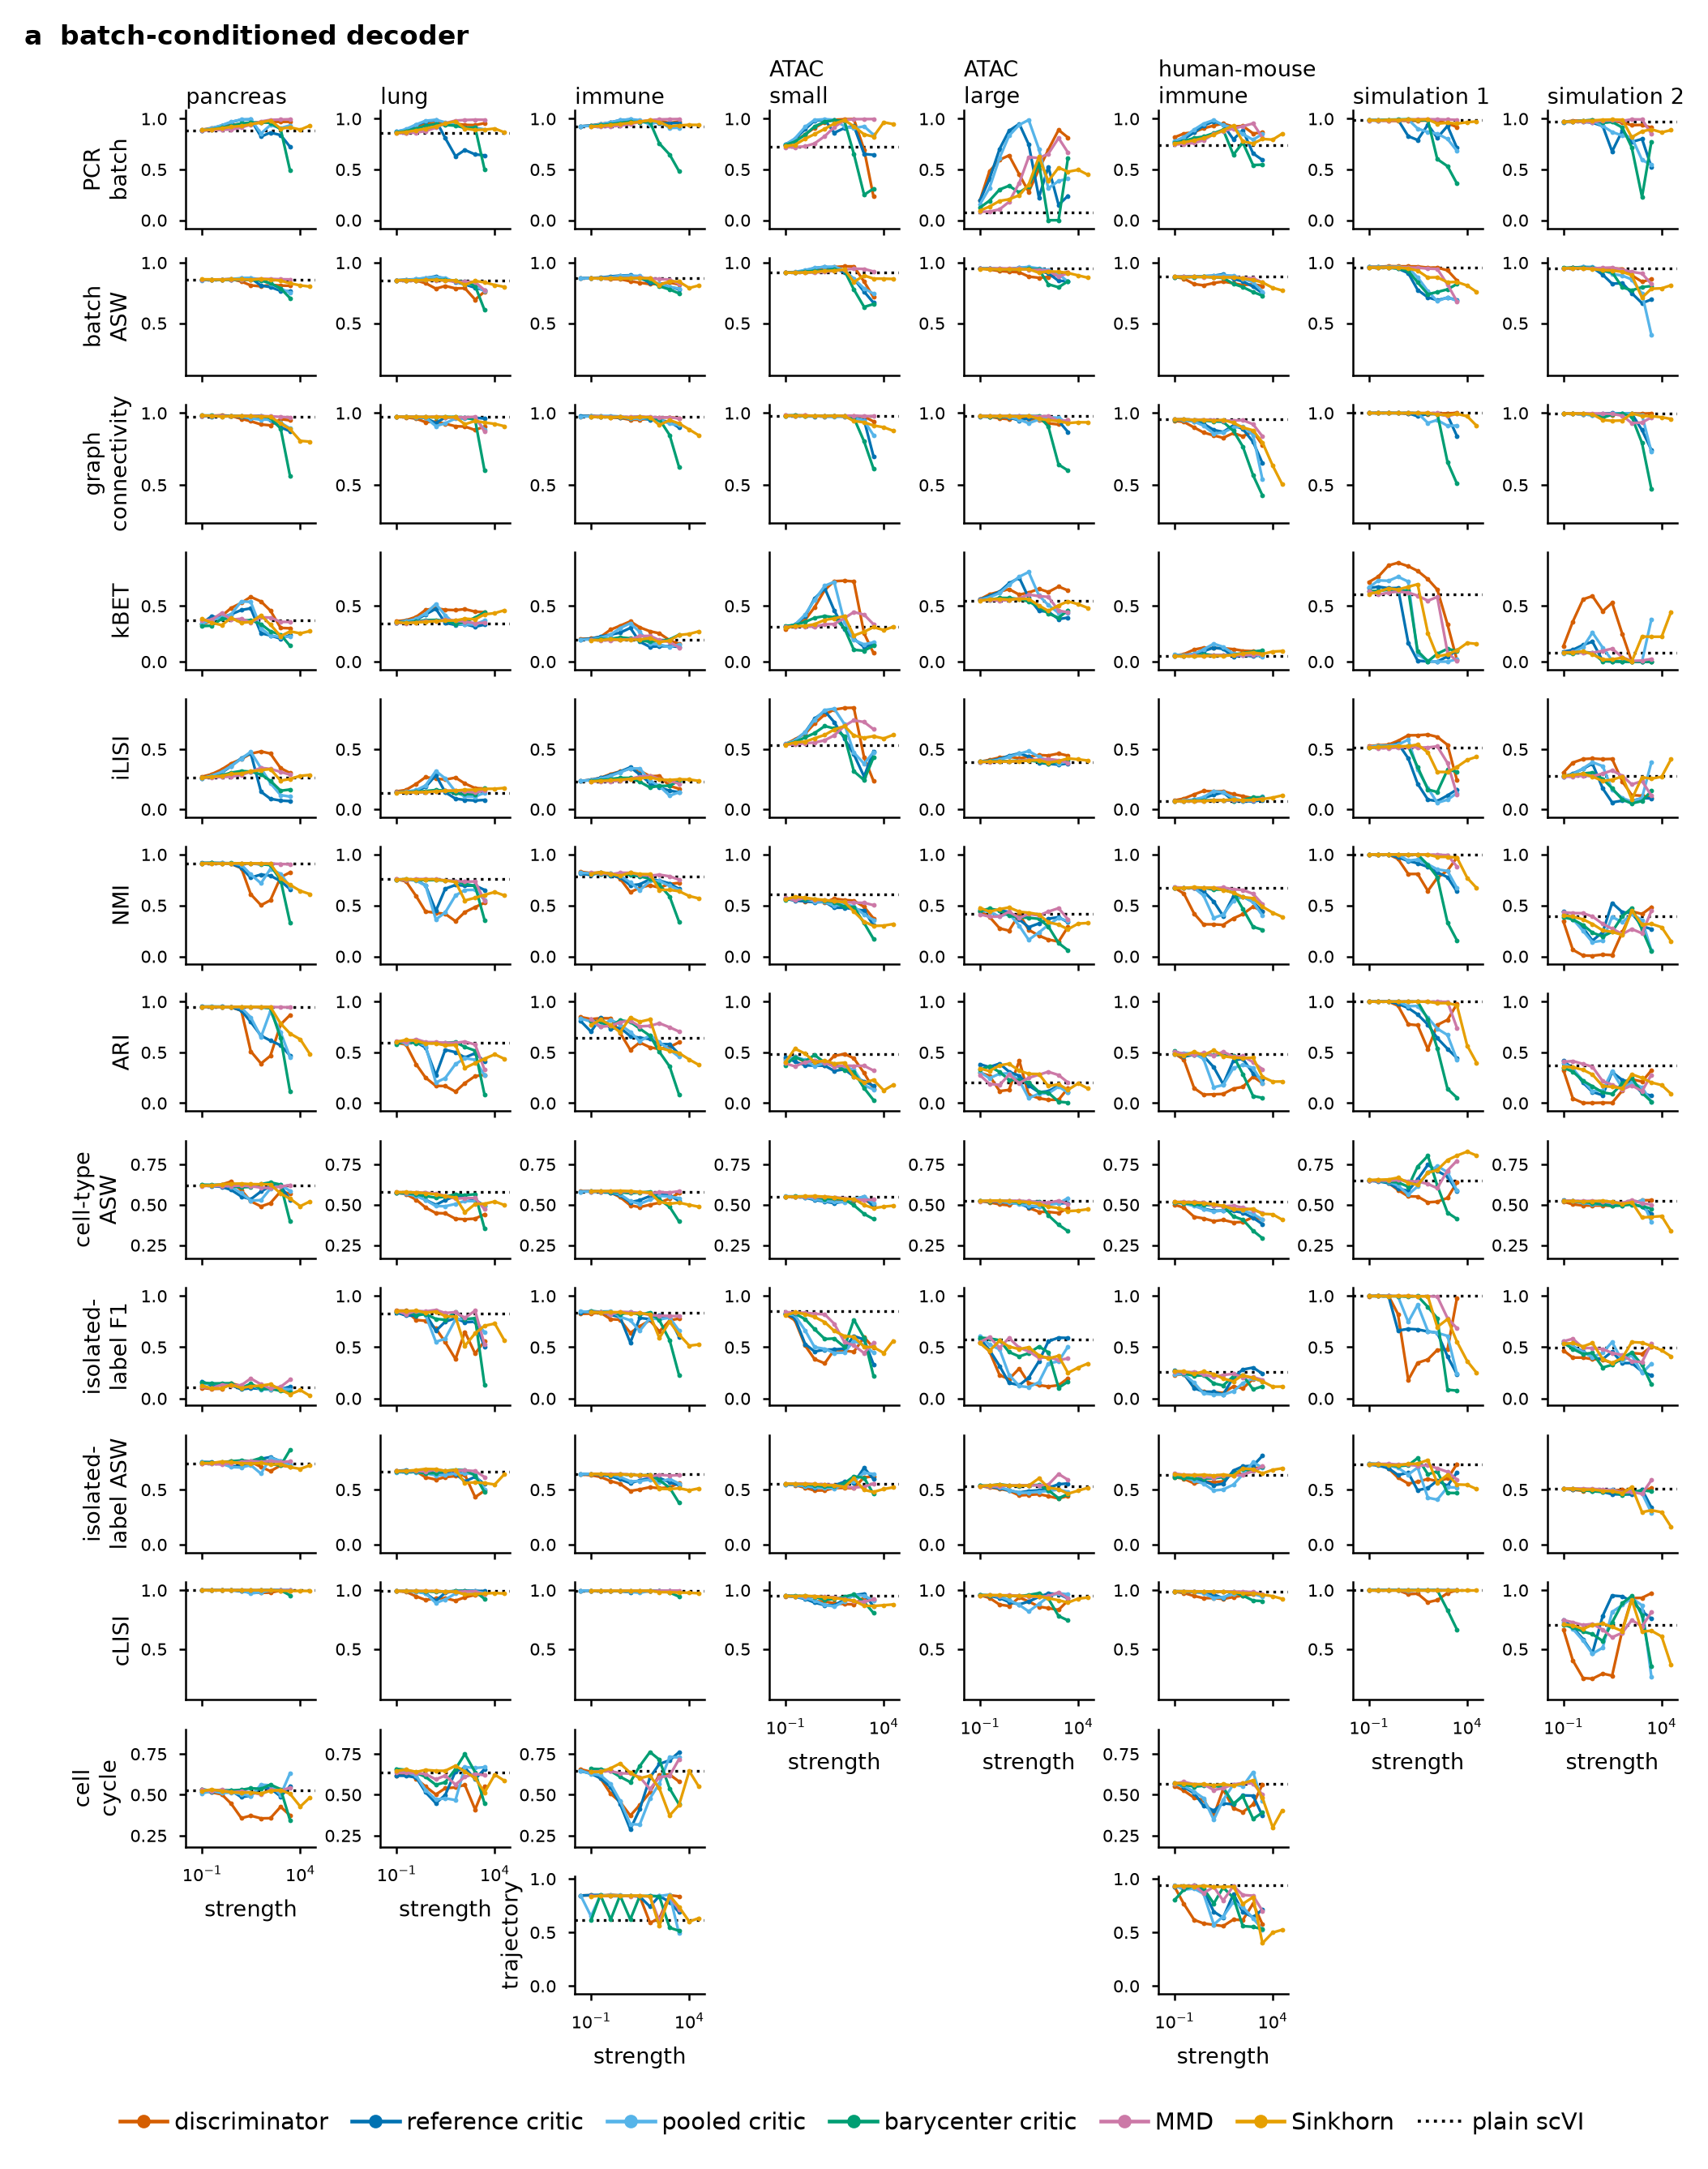
\includegraphics[width=\textwidth,height=0.78\textheight,keepaspectratio]{figures/figS4a.png}
\caption{Individual metric curves with the batch-conditioned decoder. Rows show unscaled batch metrics (1--5) and biology metrics (6--13); columns show tasks. Lines join means over three seeds against log penalty strength. Dotted lines denote plain scVI. Each row shares a vertical scale. Cell-cycle conservation applies to the four real RNA tasks and trajectory conservation to both immune tasks; other panels are empty (Supplementary Note 3).}\label{fig:s4a}
\end{figure}

\begin{figure}[p]
\centering\renewcommand{\figurename}{Supplementary Figure}\renewcommand{\thefigure}{S4b}%
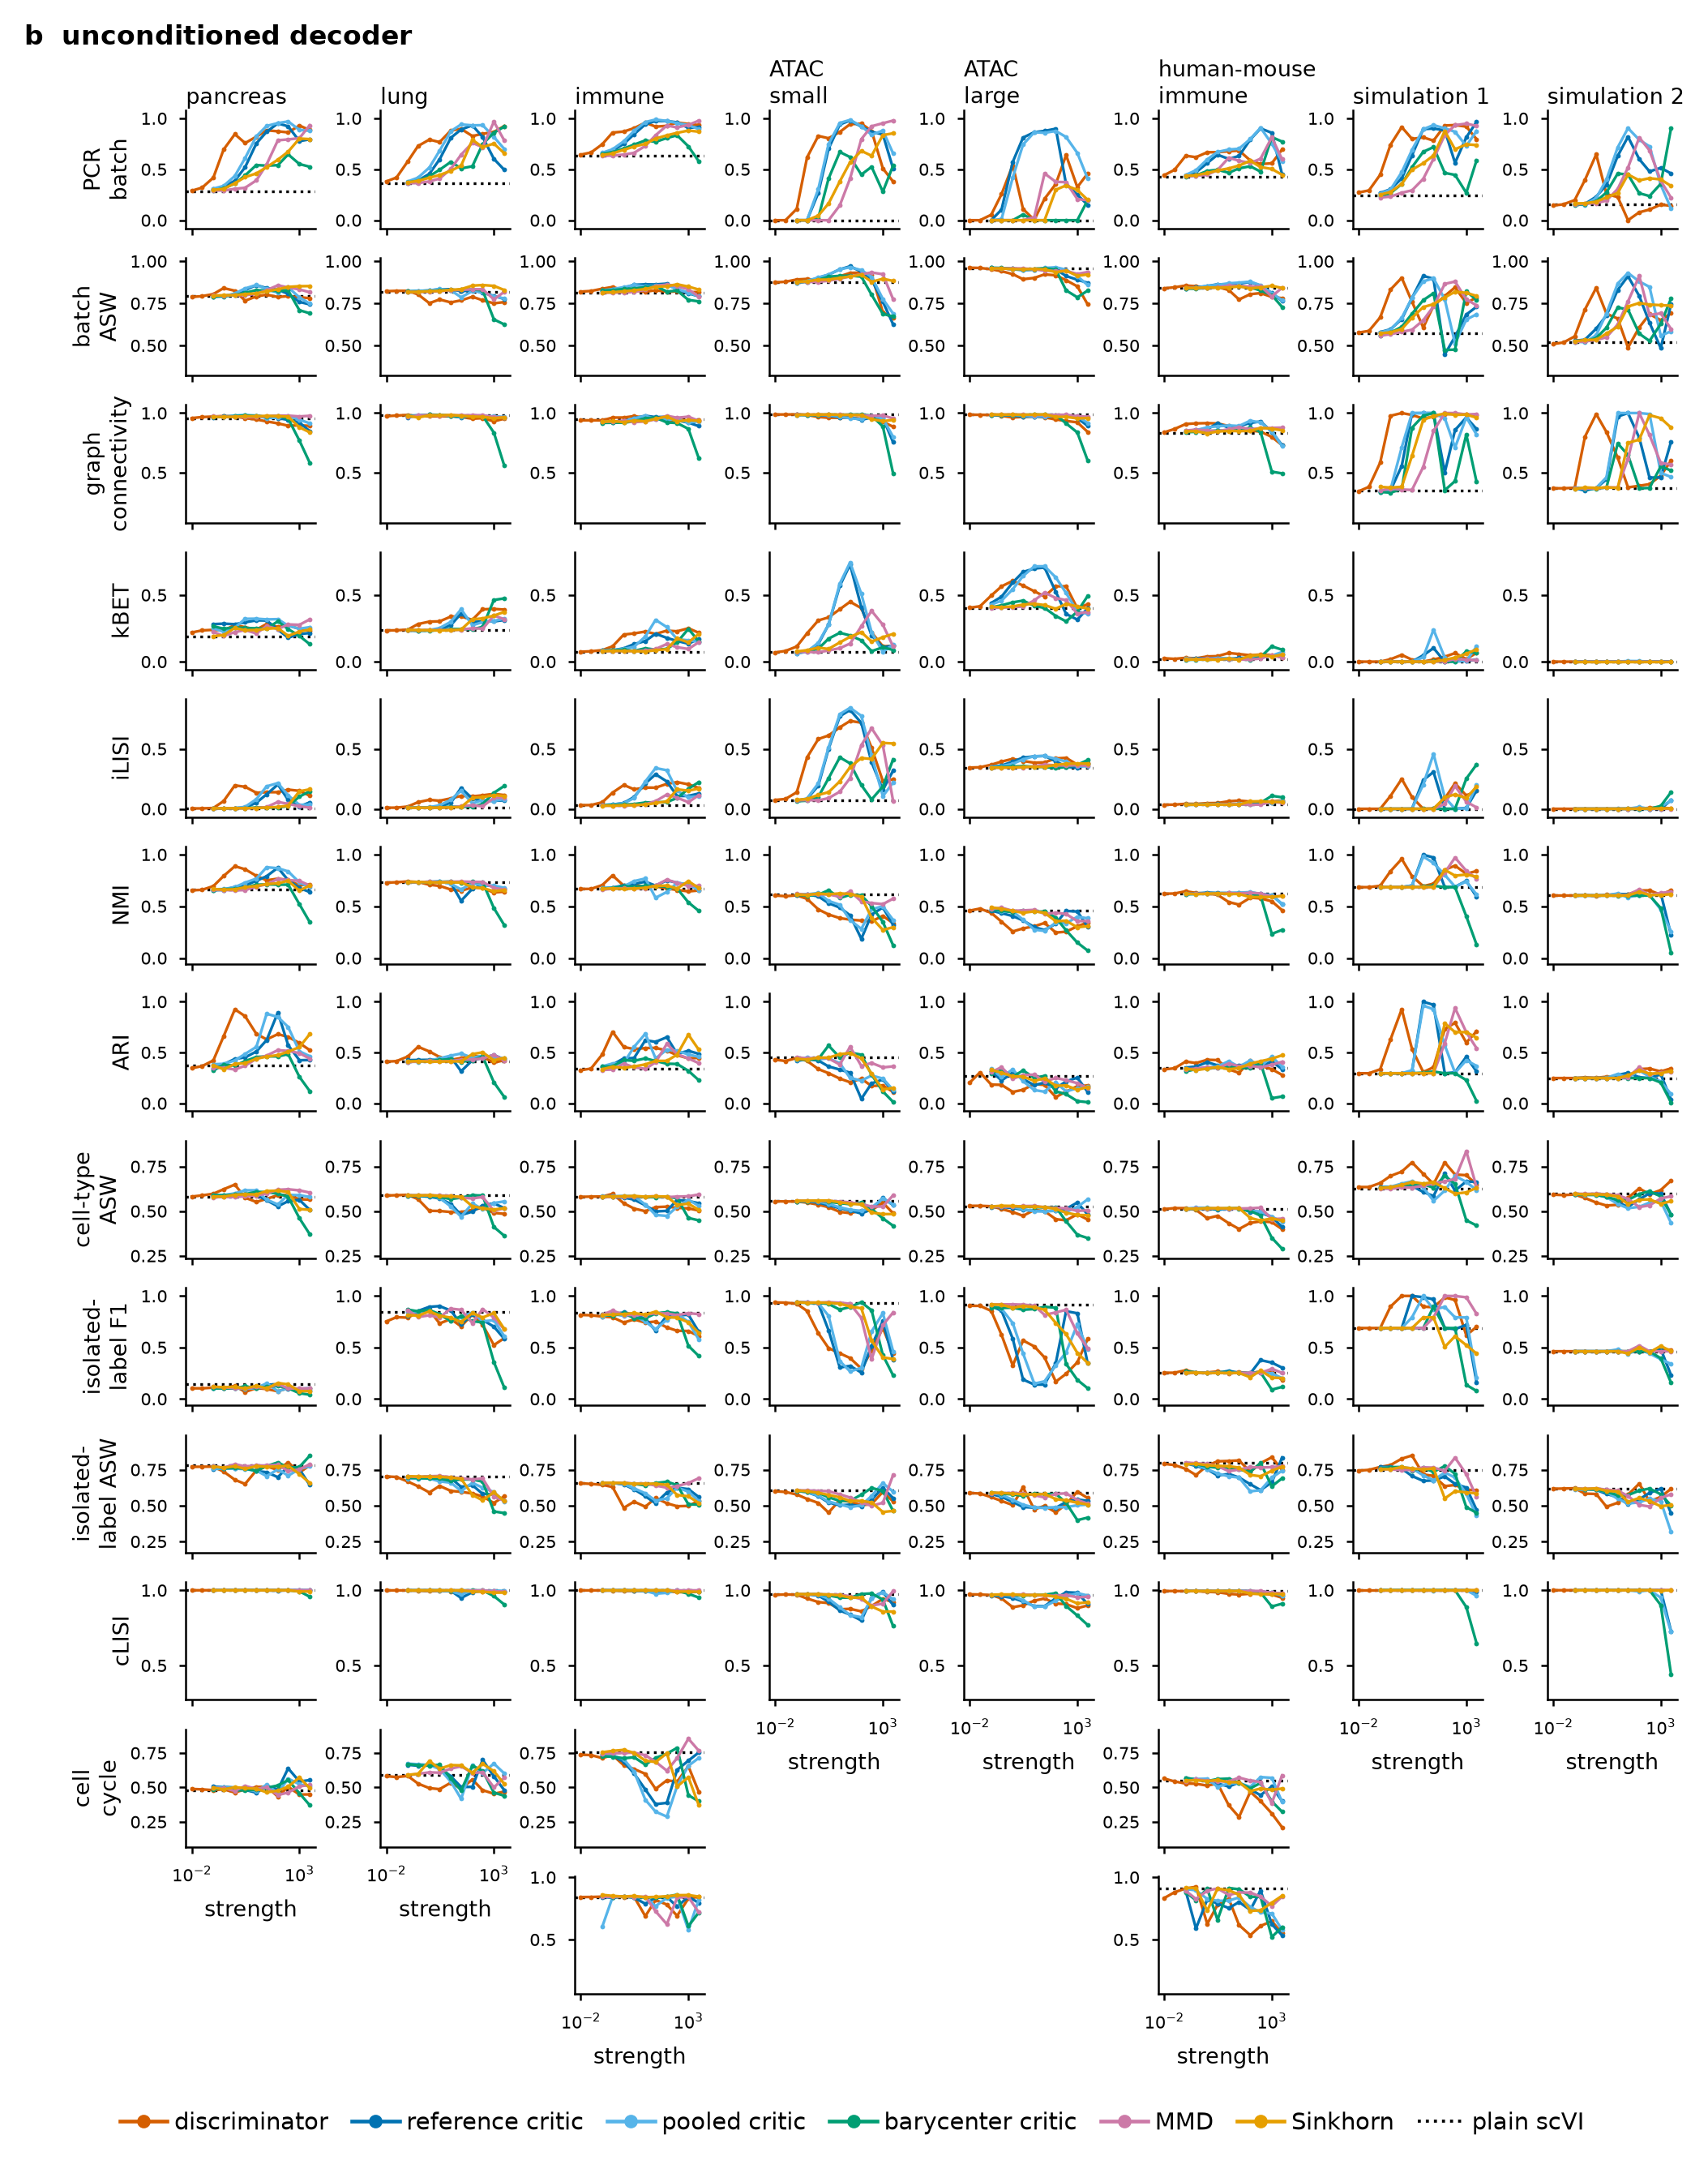
\includegraphics[width=\textwidth,height=0.78\textheight,keepaspectratio]{figures/figS4b.png}
\caption{Individual metric curves with the unconditioned decoder. Layout and definitions follow Supplementary Figure S4a.}\label{fig:s4b}
\end{figure}

\begin{figure}[p]
\centering\renewcommand{\figurename}{Supplementary Figure}\renewcommand{\thefigure}{S5}%
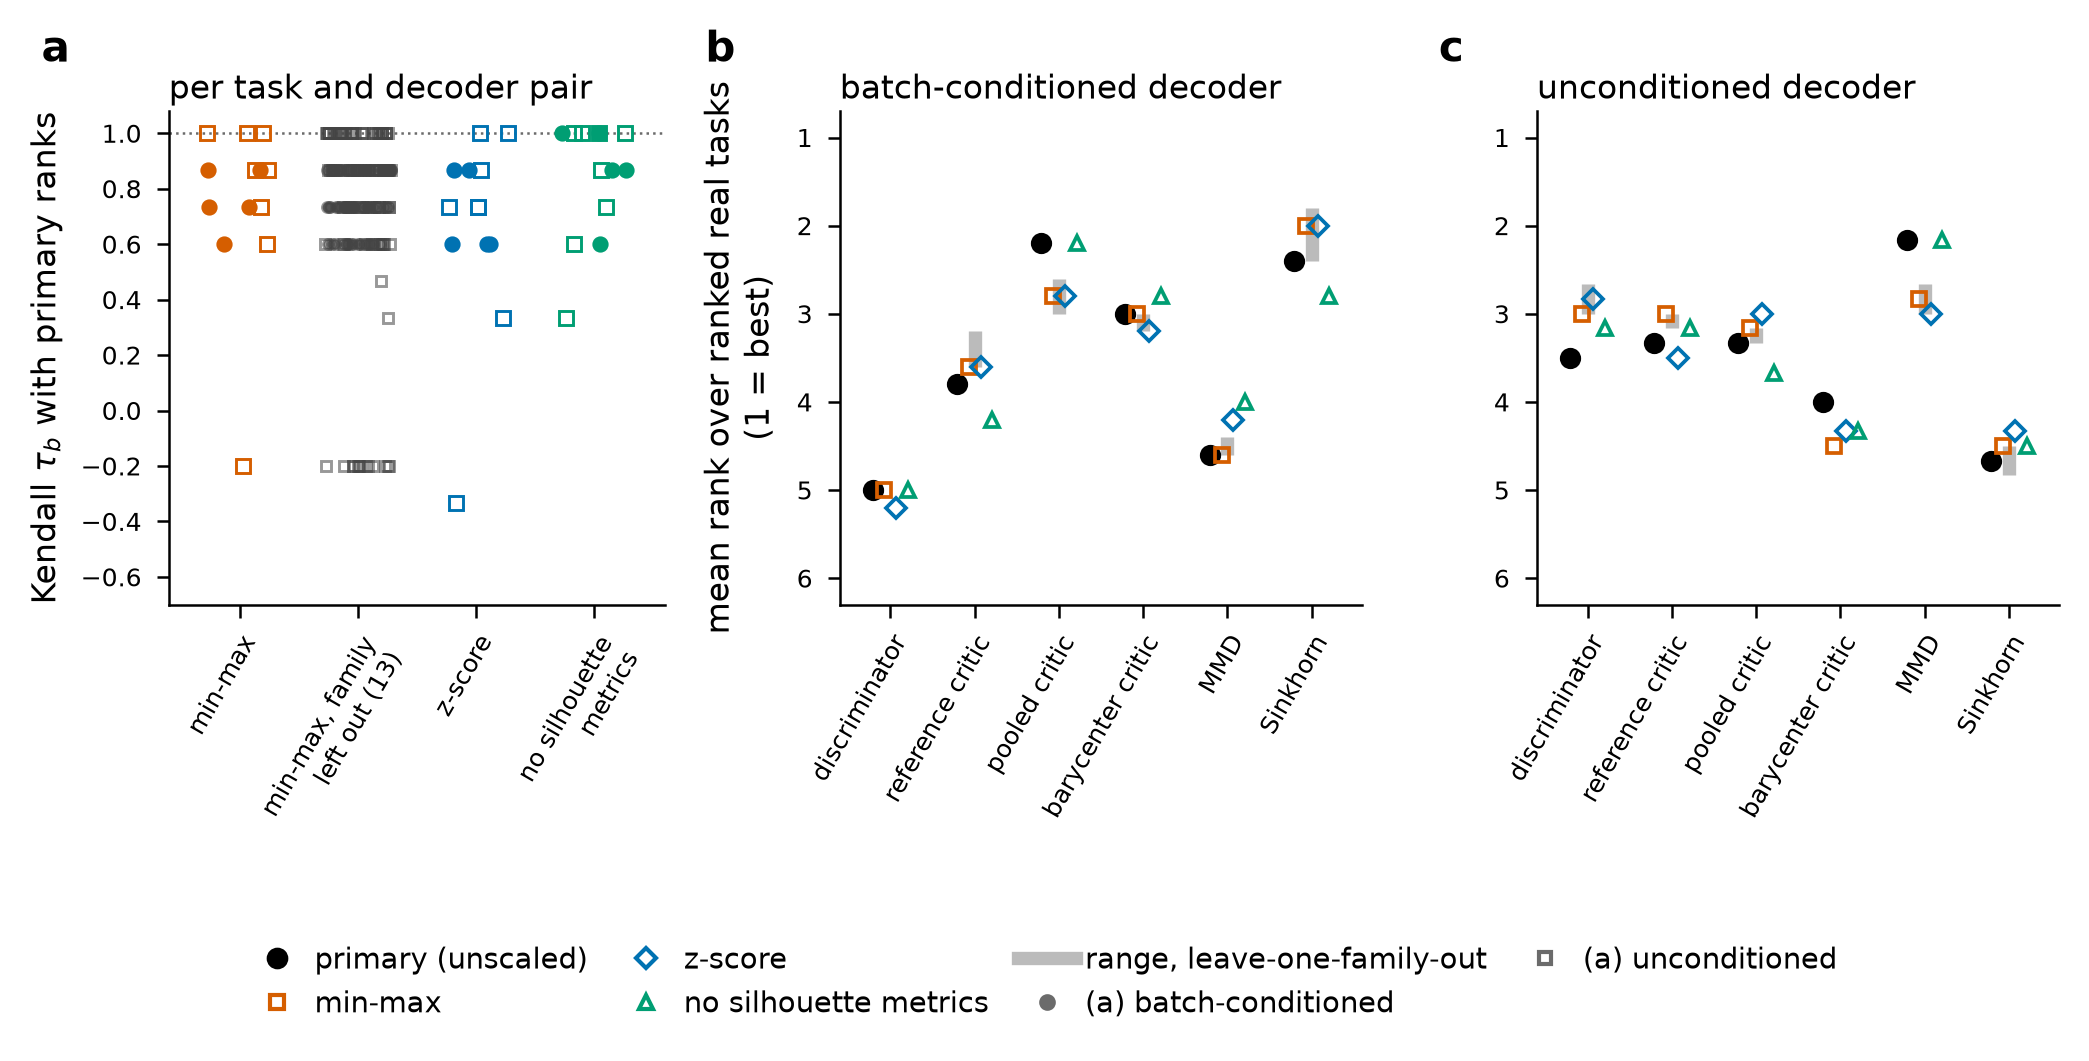
\includegraphics[width=\textwidth]{figures/figS5.png}
\caption{Sensitivity to metric scaling and composition (Supplementary Note 6). Variants use min--max scaling, omission of each method family from its scaling reference, z-scores, or exclusion of the three silhouette metrics. Scores, $b^*$ and ranks are recomputed. \textbf{(a)} Kendall's $\tau_b$ against primary rankings, with points for each ranked pair and, where applicable, omitted family. \textbf{(b, c)} Mean ranks across ranked real tasks by decoder. Grey bars span the 13 family-omission runs. Scaling can change the leading penalty.}\label{fig:s5}
\end{figure}

\begin{figure}[p]
\centering\renewcommand{\figurename}{Supplementary Figure}\renewcommand{\thefigure}{S6}%
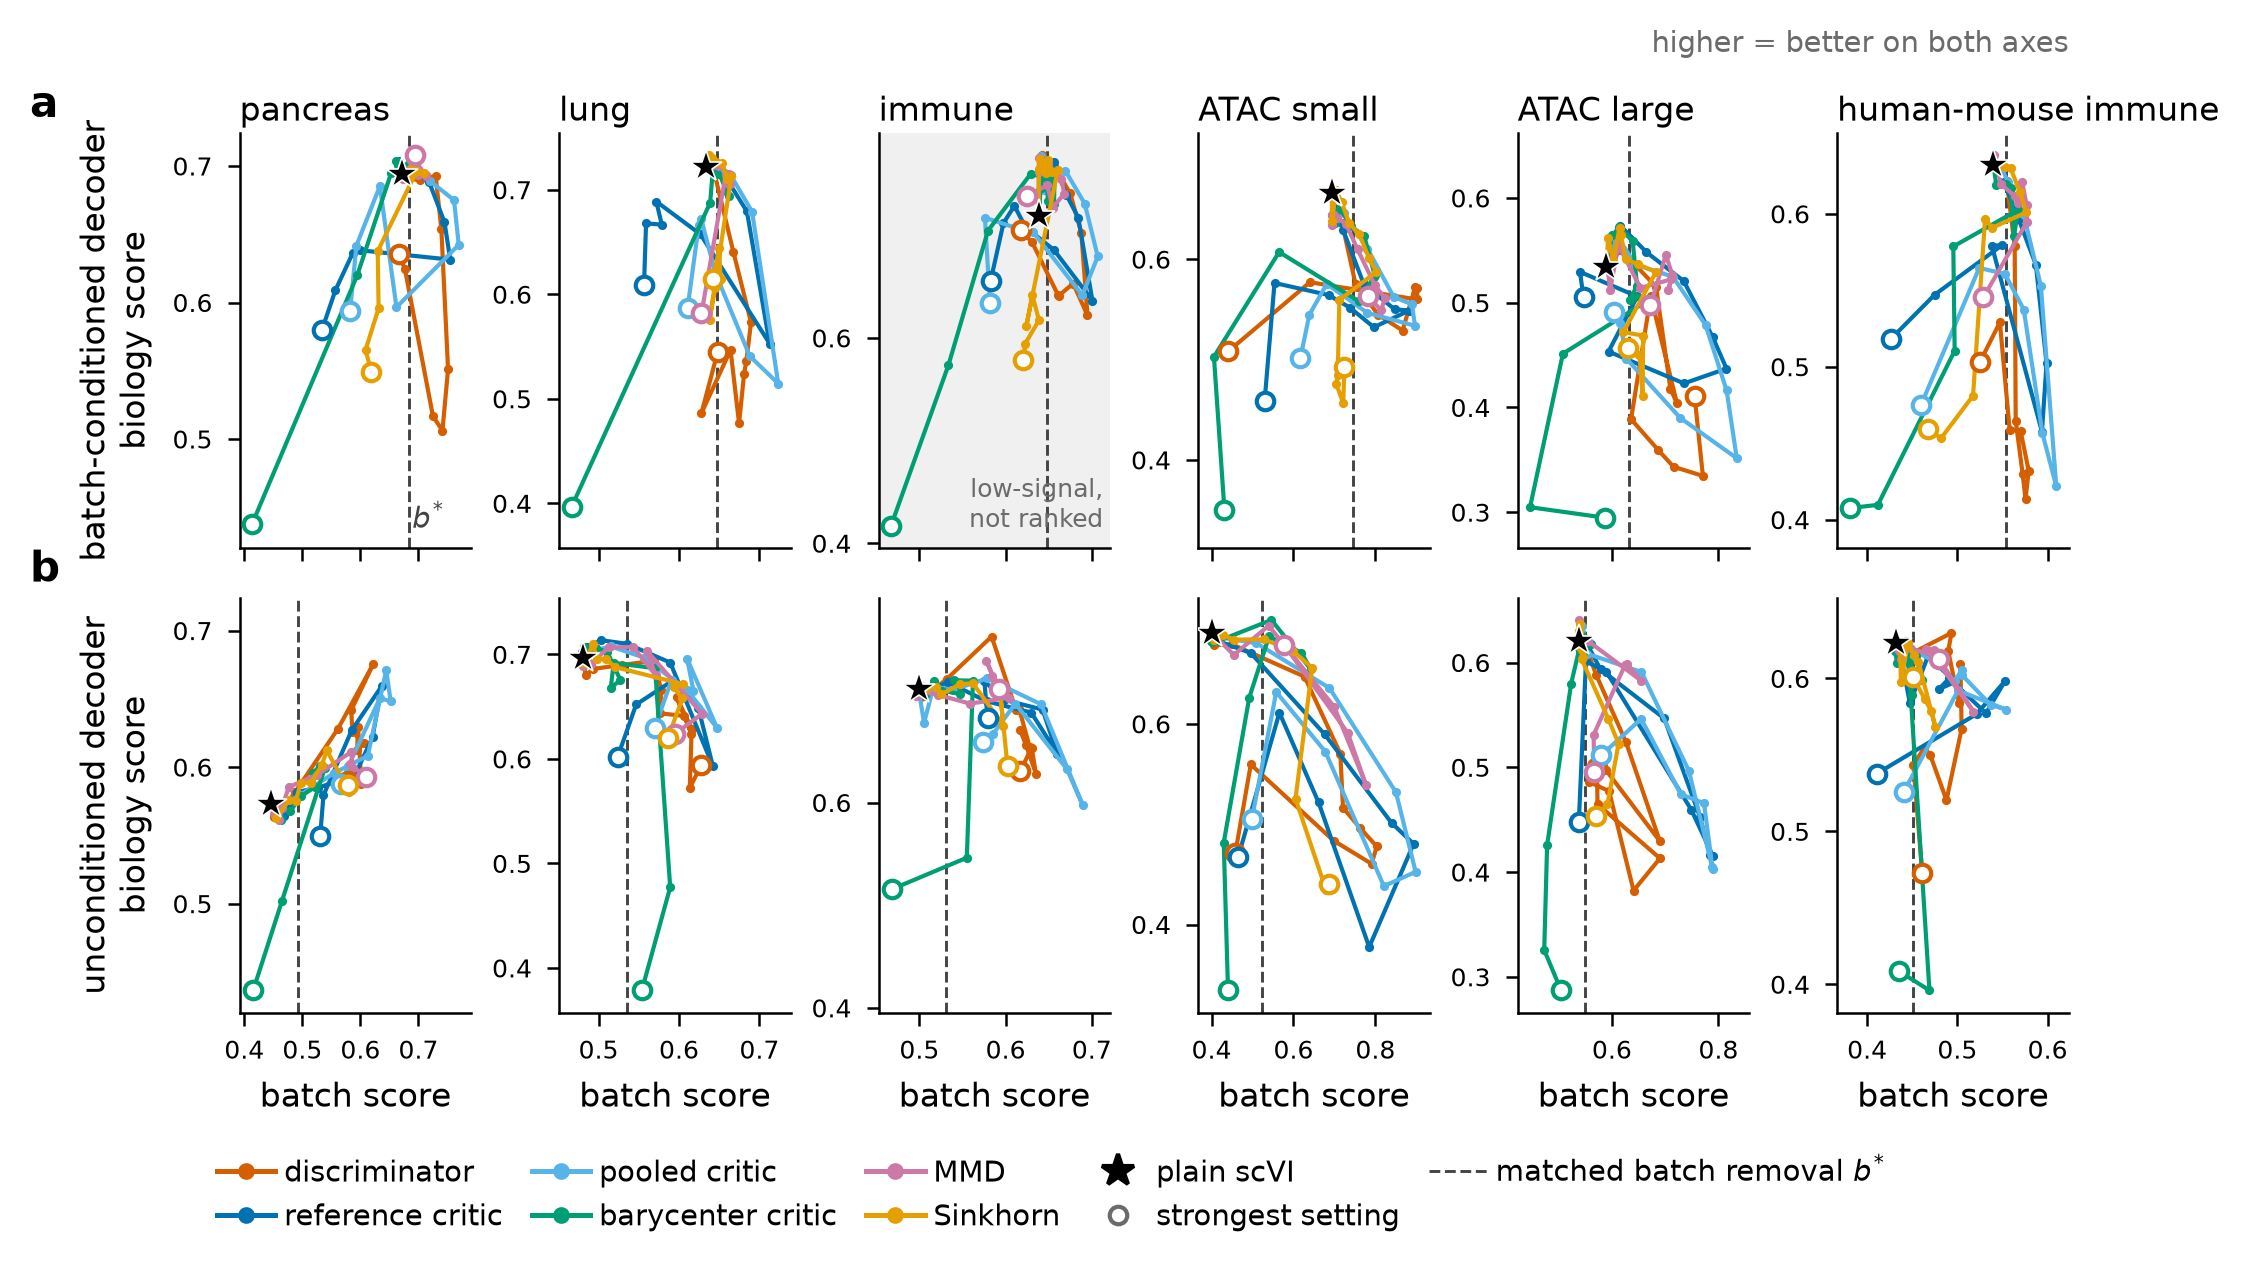
\includegraphics[width=\textwidth]{figures/figS6.png}
\caption{Trade-off curves for six real tasks with batch-conditioned \textbf{(a)} and unconditioned \textbf{(b)} decoders. Lines join seed-mean scores from plain scVI (star) through increasing penalty strengths. Open circles mark strongest settings; dashed lines mark $b^*$. Grey identifies the low-signal immune pair. Panels within columns share axes. Supplementary Figure S7 compares biology at $b^*$ and at the strongest setting.}\label{fig:s6}
\end{figure}

\begin{figure}[p]
\centering\renewcommand{\figurename}{Supplementary Figure}\renewcommand{\thefigure}{S7}%
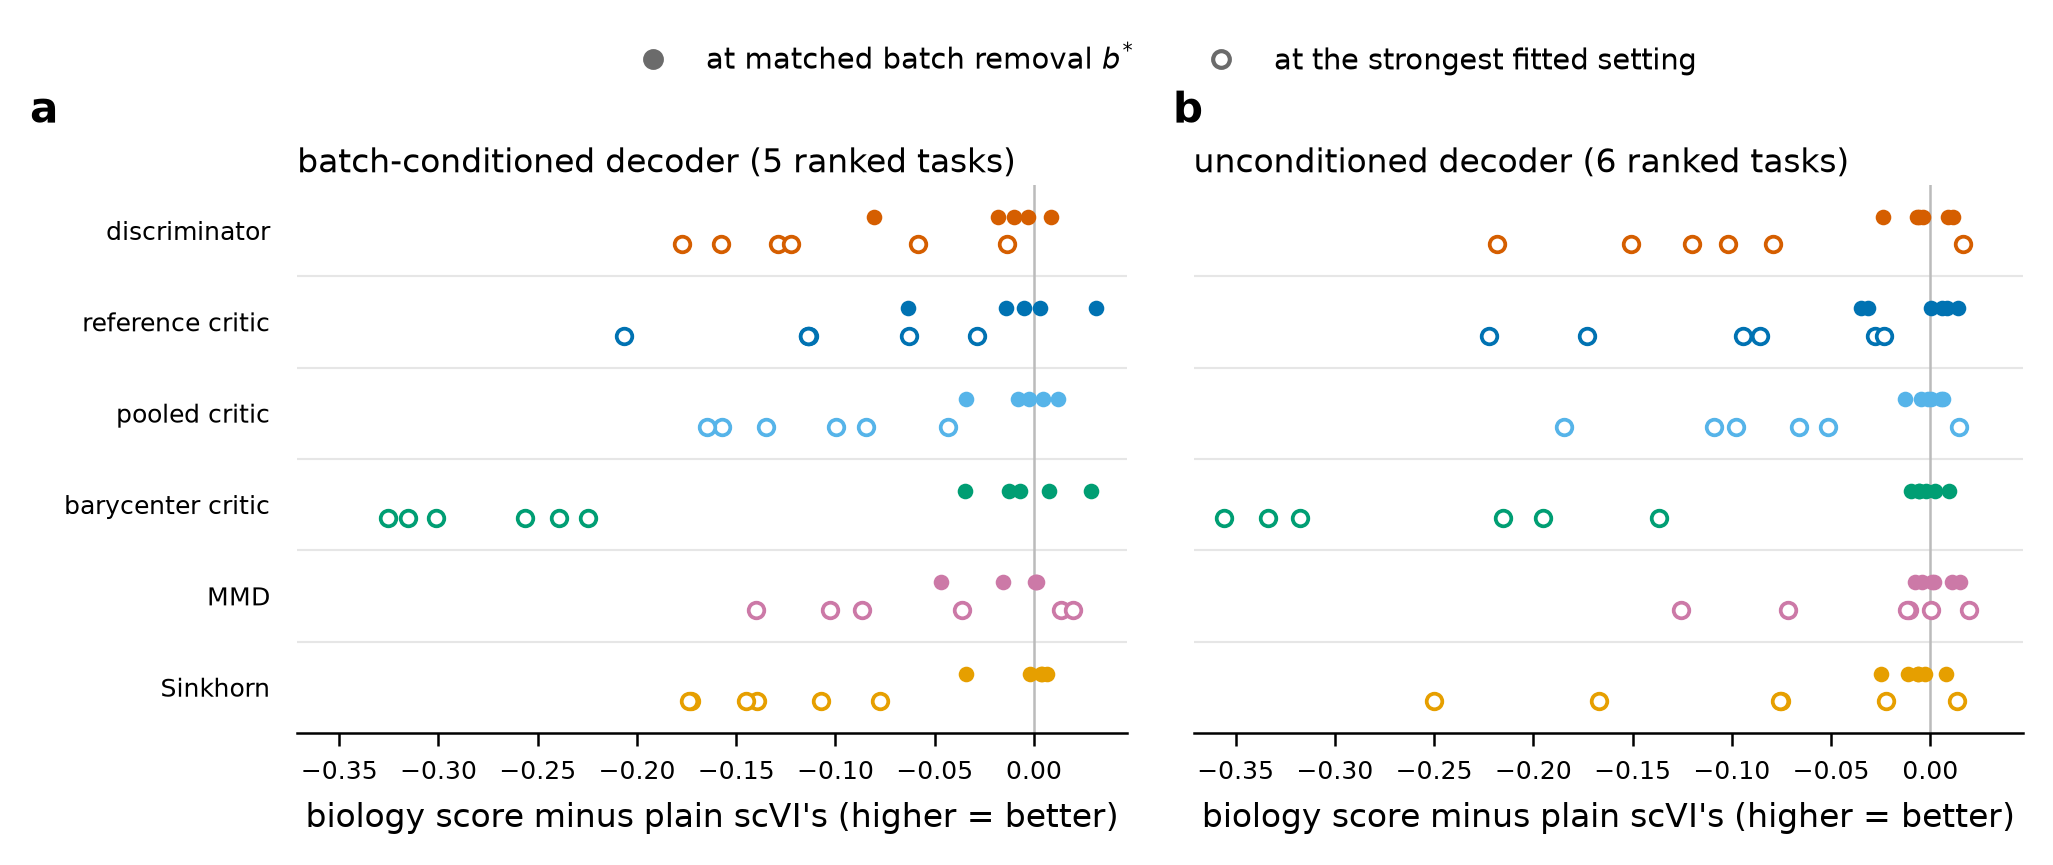
\includegraphics[width=\textwidth]{figures/figS7.png}
\caption{Biology differences from same-decoder plain scVI at $b^*$ (filled dots) and the strongest fitted setting (open dots). Panels show batch-conditioned \textbf{(a)} and unconditioned \textbf{(b)} decoders. Each dot represents a real task; grey marks no change. Filled dots exclude the low-signal immune pair, while open dots include all tasks. Supplementary Figure S6 gives full curves.}\label{fig:s7}
\end{figure}

\begin{figure}[p]
\centering\renewcommand{\figurename}{Supplementary Figure}\renewcommand{\thefigure}{S8}%
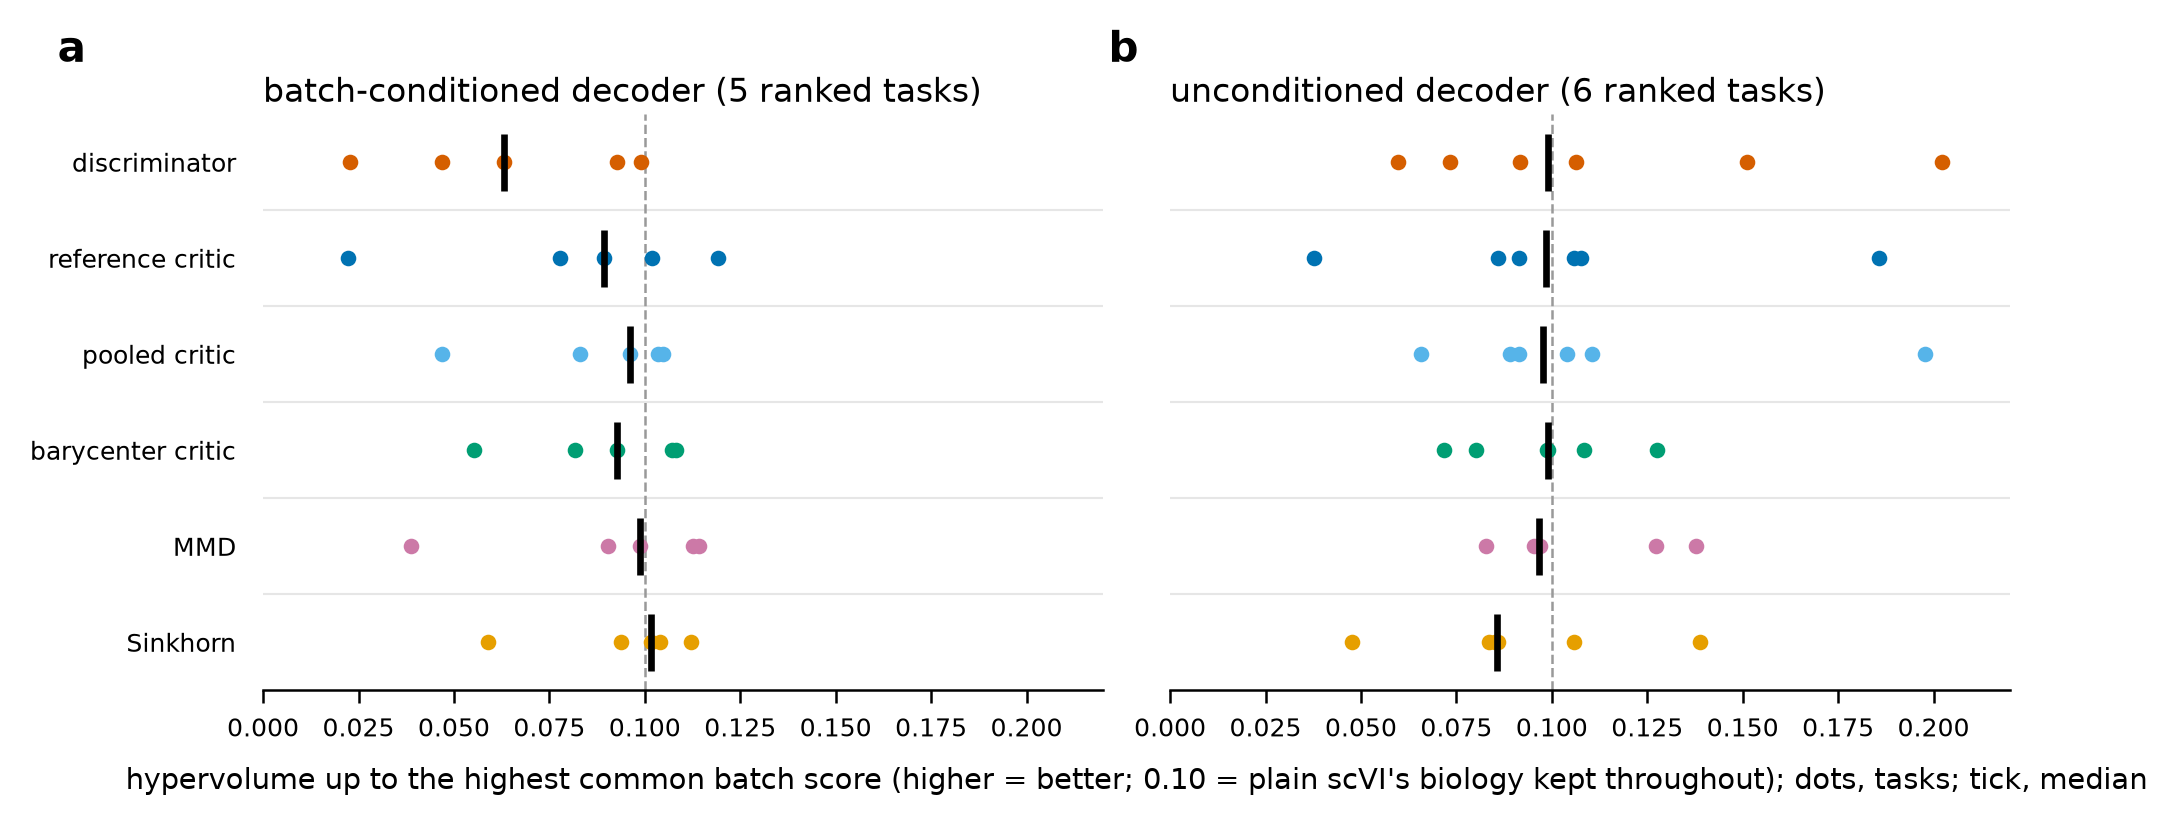
\includegraphics[width=\textwidth]{figures/figS8.png}
\caption{Hypervolume capped at the highest common batch score, with batch-conditioned \textbf{(a)} and unconditioned \textbf{(b)} decoders. Dots represent ranked real tasks and black ticks their median. The area lies under each Pareto frontier above biology difference $-0.10$, divided by the common batch gap. The dashed value 0.10 denotes retention of plain-scVI biology throughout. Supplementary Note 7 defines the measure; Supplementary Table S8 also gives uncapped values.}\label{fig:s8}
\end{figure}

\begin{figure}[p]
\centering\renewcommand{\figurename}{Supplementary Figure}\renewcommand{\thefigure}{S9}%
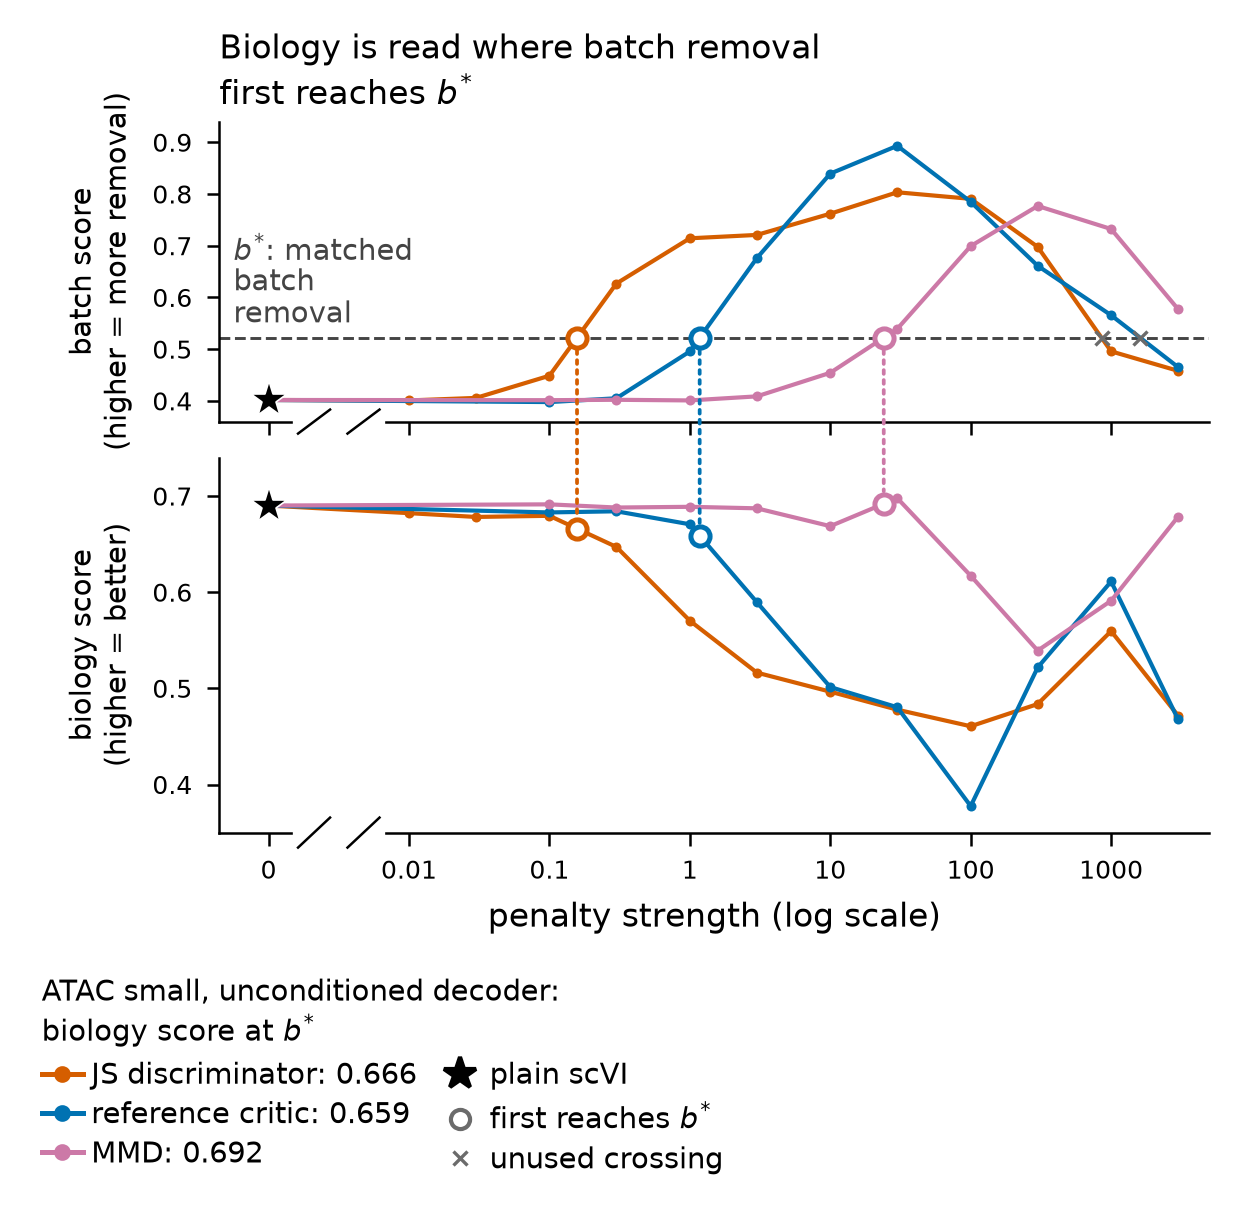
\includegraphics[width=0.6\textwidth]{figures/figS9.png}
\caption{Reading biology at $b^*$ on unconditioned ATAC small for the discriminator, reference critic and MMD. Curves show mean scores over seeds 100--102 against log strength, with plain scVI at 0 beyond the axis break. Open circles bracket the first crossing of dashed $b^*$; dotted segments show interpolation in batch score. Later crossings, marked by grey crosses, are ignored. The legend gives biology at $b^*$ (Supplementary Note 5).}\label{fig:s9}
\end{figure}
